

\documentclass{beamer}

\usepackage{simlab}

% Replace short paper title (inside square brackets) by our lab name
\title[Artifical Neural Networks]
{}

%\subtitle{Include Only If Paper Has a Subtitle}

% Give the names in the same order as they appear in the paper.
% Use the \inst{?} command only if the authors have different affiliation.
% Names inside square brackets will appear at the bottom of each slide.
\author[Mitchell Corbett/Matthew Galbraith]{Mitchell Corbett}



% Uncomment this if you want the table of contents to pop up at the beginning of
% each subsection:
%\AtBeginSubsection[] {
%  \begin{frame}<beamer>
%  \frametitle{Outline}
%  \tableofcontents[currentsection,currentsubsection]
%  \end{frame}
%}

\begin{document} 
 
% If you wish to uncover everything in a step-wise fashion, uncomment the
% following command: 
%\beamerdefaultoverlayspecification{<+->}



% Comment the following lines if you wish to hide frame number
\expandafter\def\expandafter\insertshorttitle\expandafter{%
  \insertshorttitle\hfill%
  \insertframenumber\,/\,\inserttotalframenumber}

\begin{frame}
  \frametitle{Outline}
  \tableofcontents[pausesections]
  % You might wish to add the option [pausesubsections] as well.
\end{frame}

%---------------------------------------------------------------------- SECTION
\section{Introduction to ANN}
\begin{frame}
\frametitle{What is a Neural Network?}

\begin{itemize}
	\item The question "What is a Neural Network" is somewhat ill posed.
    
\end{itemize}
\end{frame}
\subsection{Biological Inspirations}
\begin{frame}
\frametitle{Biological Inspirations}
\begin{itemize}
	\item In Biology, the Neuron is a fundamental unit of the Central Nervous System. It contains 3 parts. The Cell Body, Dendrites, and an Axon.
	\begin{itemize}
		\item The Cell Body contains the essential parts of the cell
		\item Dendrites are short fibers that receive signals.
		\item The Axon is a long projecting branch which sends signals. It can branch in to many other cells.
\end{itemize}
\end{itemize}
\end{frame}
\begin{frame}
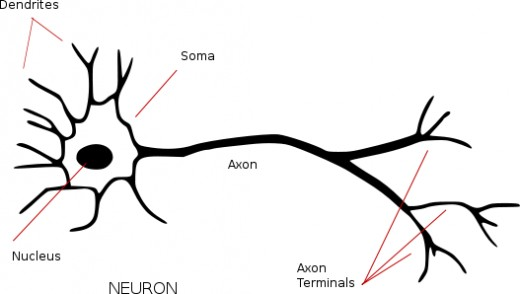
\includegraphics[width = 350px]{neuron.jpg}
\end{frame}

\subsection{Different Definitions}
\begin{frame}
\frametitle{DARPA NN Study}
\begin{itemize}
	\item "...a Neural Network is a system composed of many simple processing elements operating in parallel whose function is determined by network structure, connection strength and the processing performed at computing elements or nodes"
\end{itemize}
\end{frame}

\begin{frame}
\frametitle{Haykin (1994)}
\begin{itemize}
\item A neural network is a massively parallel distributed processor that has a natural propensity for storing experiential knowledge and making it available for use. It resembles the brain in two respects: 
  Knowledge is acquired by the network through a learning process. 
  Interneuron connection strengths known as synaptic weights are used to store the knowledge.
\end{itemize}
\end{frame}
\subsection{Applications}
\begin{frame}
\begin{itemize}
\item Classification
\end{itemize}
\end{frame}

\begin{frame}
\begin{itemize}
\item With that, let's dive in!
\end{itemize}
\end{frame}

\section{Feed-Forward Neural Networks}
\subsection{Model of an "Artifical" Neuron}
\begin{frame}
\frametitle{What the heck is a Neuron}
\begin{itemize}
	\item We need to discuss how we can model a Neuron computationally. 
    \item A basic neuron has 3 key components. \textbf{Synapses}, an \textbf{Adder}, and an \textbf{Activation Function}.
\end{itemize}

\end{frame}

\begin{frame}
\frametitle{Components of a Basic Neuron}
\begin{block}{Synapses}
Synapses or "Links" which each have a weight assigned to them. If we have an input signal coming in to a neuron, we will want to weight them differently.
\end{block}
\begin{block}{Adder}
Used for summing the input signals which have been weighted. 
\end{block}

\begin{block}{Adder}
is used to limit the output of a neuron. Essentially what the activation function does is require that a sufficiently strong output is reached. This is very similar to the neurons in our brains, which fire or activate in response to a change in electrical charge.
\end{block}

\end{frame}









\end{document}